\documentclass{beamer}
\usepackage{pdfpages}
\usepackage{tabularx}
\usepackage{array}
\usepackage{booktabs}
\usepackage{listings}
\usepackage{tikz-timing}

\definecolor{darkgreen}{HTML}{008000}
\lstset{frame=single,
    language=Haskell,
    breaklines=true,
    showspaces=false,
    showstringspaces=false,
    showtabs=false,
    basicstyle=\footnotesize,
    commentstyle=\color{darkgreen},
    keywordstyle=\color{blue},
    stringstyle=\color{purple},
}
\def\tabularxcolumn#1{m{#1}}
\pagenumbering{roman}
\tikzset{timing/draw grid}

%Beamer settings
\usetheme{Frankfurt}

%Disable Figure: prefix
\setbeamertemplate{caption}{\insertcaption}
\setbeamertemplate{caption label separator}{}

\AtBeginSection{\frame{\sectionpage}}

\title{H2V --- a Haskell to Verilog Compiler}
\author{Reuben D'Netto (22096620)}
\date{30th October 2014}
\institute{Supervised by: David Boland}

\begin{document}
\frame{\titlepage}

\begin{frame}
    \frametitle{Significant Contributions}
    \begin{itemize}
        \item Designed and implemented a Haskell to Verilog compiler, with support for the following language features:
            \begin{itemize}
                \item Pattern matching
                \item Pattern guards
                \item Tail-recursive functions
                \item Higher-order functions (evaluated at compile-time)
                \item Partial application
            \end{itemize}
        \item Designed and implemented support for the following functions through a combination of generated and hard-coded Verilog:
            \begin{itemize}
                \item List operators: cons (:), concat (++)
                \item Higher-order list functions: map, fold/reduce, zipWith
            \end{itemize}
        \item Designed and implemented support for N-degree parallel computation of lists, as defined by user
        \item Designed and implemented data flow graph generation
        \item Verified hardware generated for test cases using SignalTap
    \end{itemize}
\end{frame}

{% Include poster
\setbeamercolor{background canvas}{bg=}
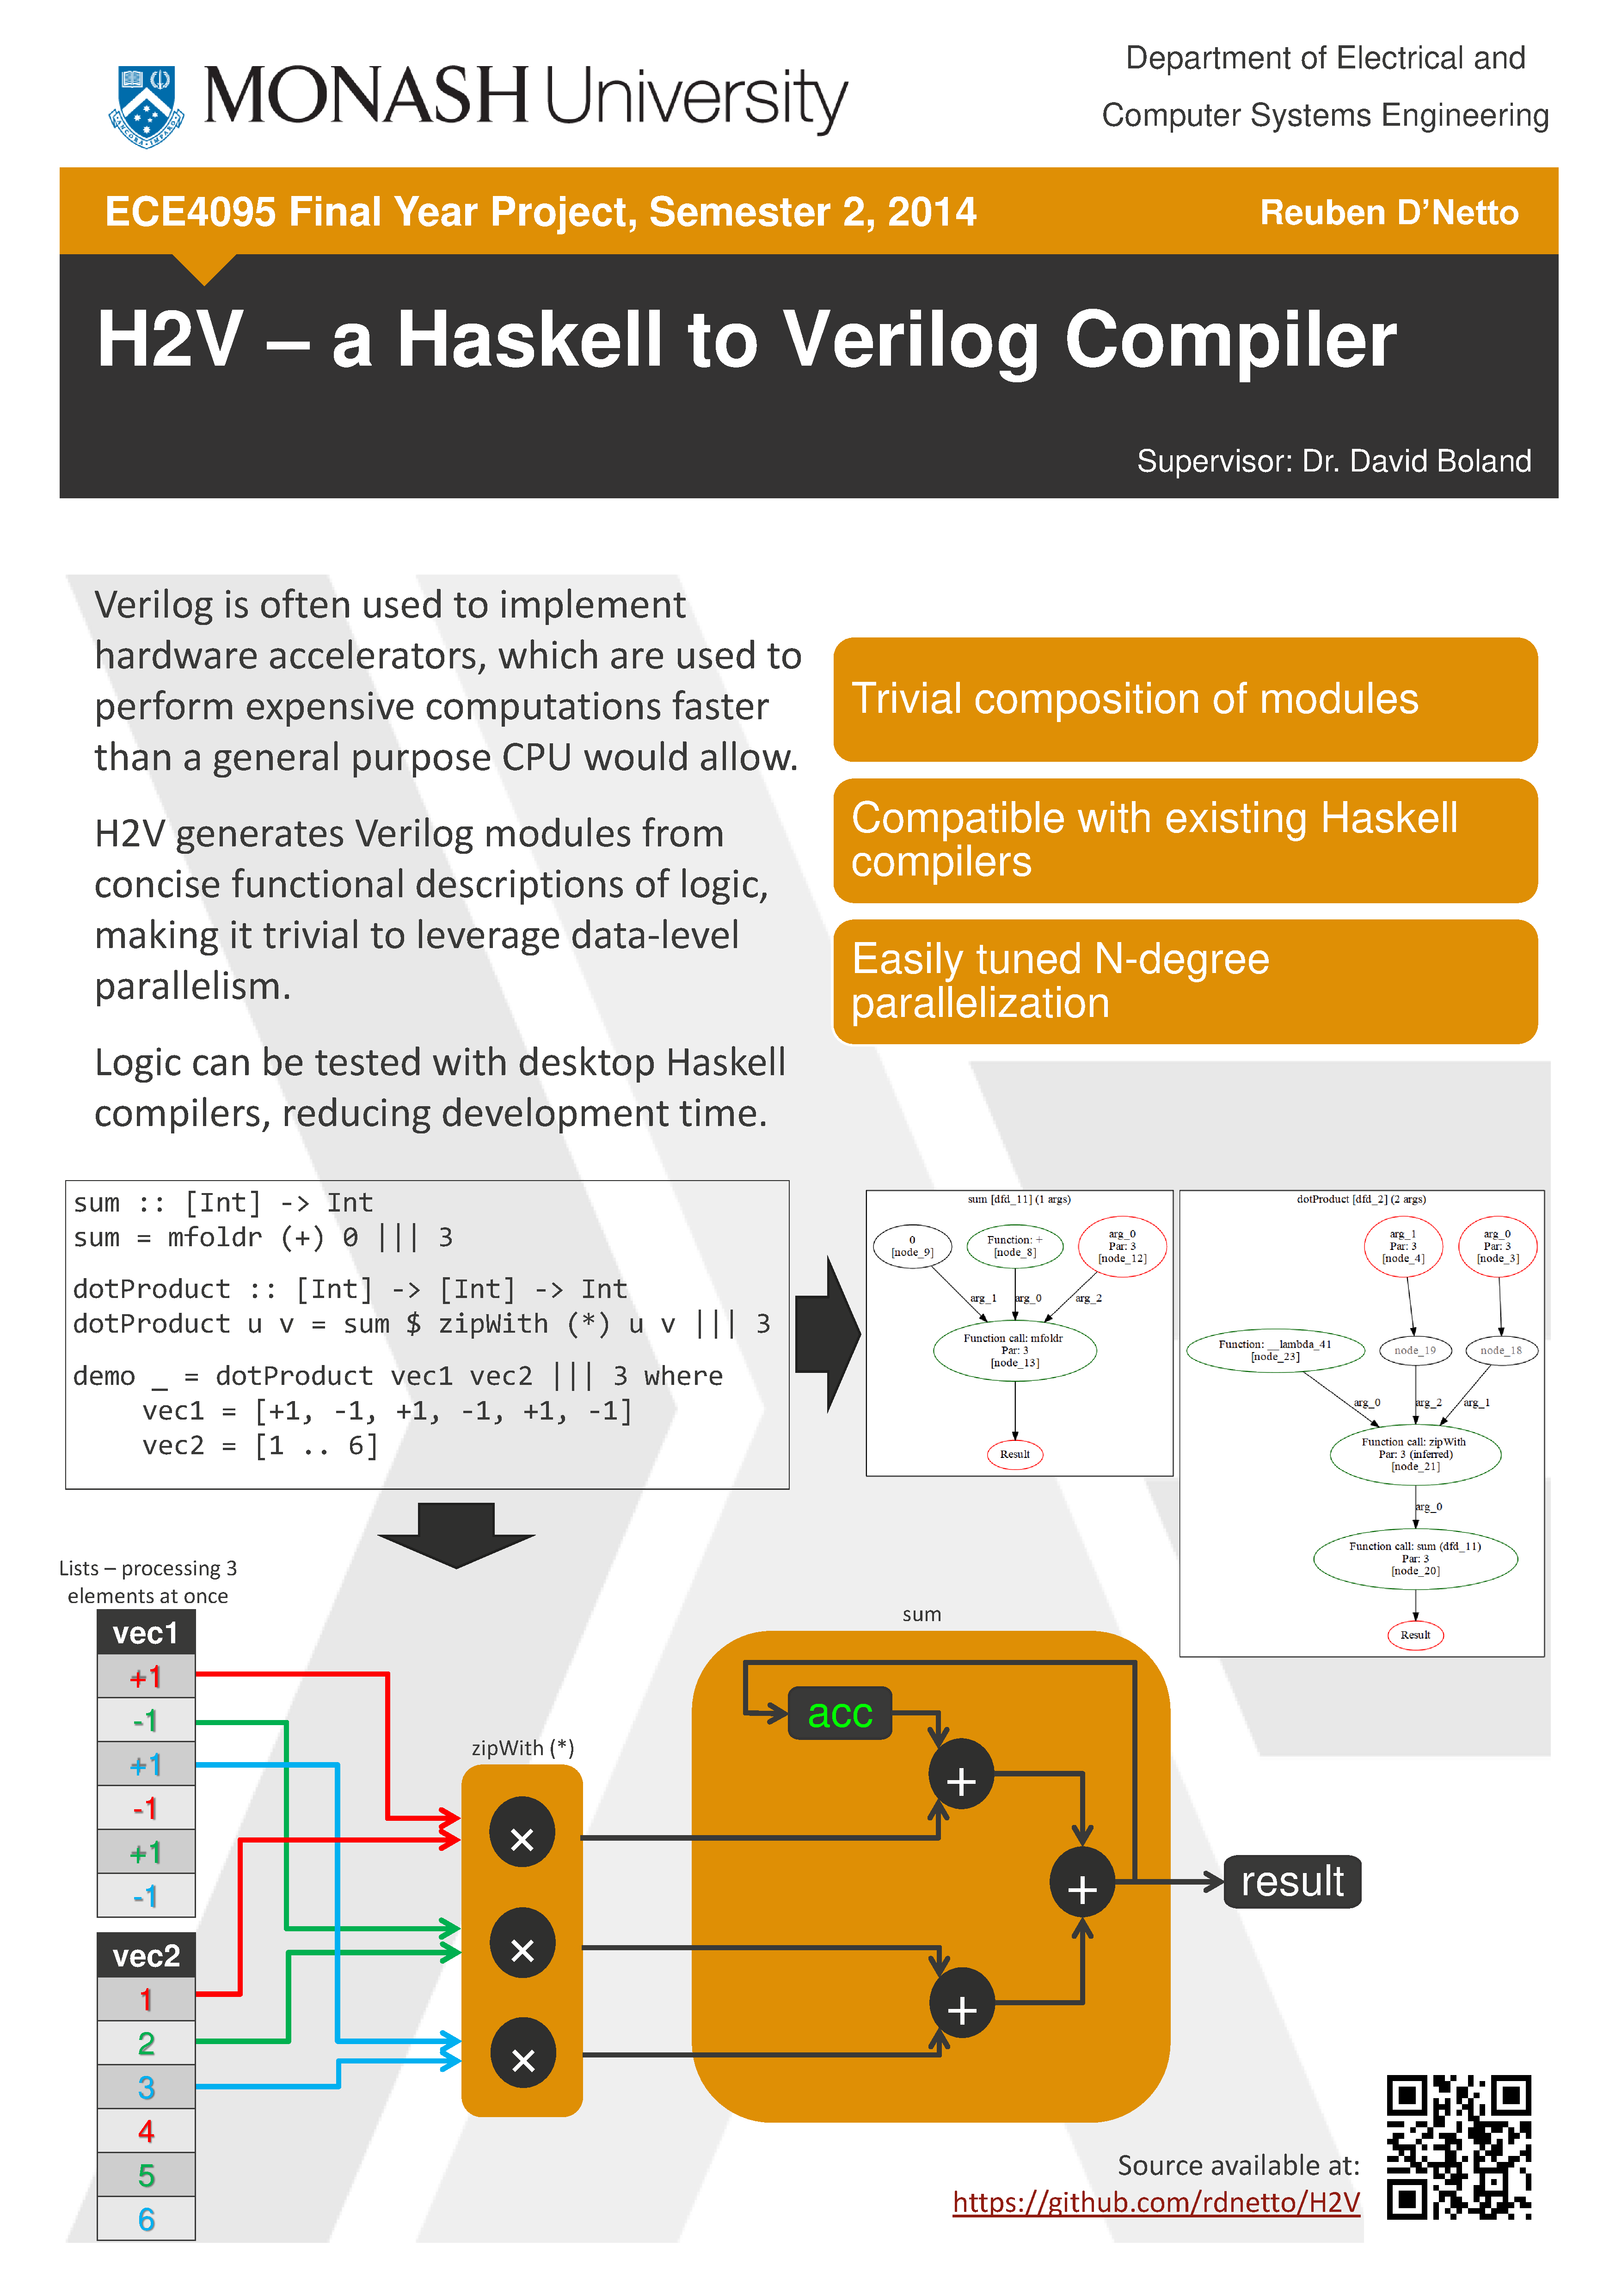
\includepdf[pages={1}]{../Poster/Poster.pdf}
}


\section{Introduction}

\begin{frame}[t]
    \frametitle{Introduction}
    \begin{itemize}
        \item Verilog
            \begin{itemize}
                \item Interfacing with digital integrated circuits
                \item Accelerating expensive computations
            \end{itemize}
        \item Haskell
            \begin{itemize}
                \item Pure
                \item Functional
                \item Concise
            \end{itemize}
        \item Proof of concept
    \end{itemize}
\end{frame}


\begin{frame}[fragile]
    \frametitle{Purity is good for optimization!}
    \begin{block}{Pure function}
        A function whose result does not depend on any shared or global state. Modifications to such state are referred to as
        \textit{side-effects}.
    \end{block}

    \lstinputlisting{src/intro.hs}
    \lstinputlisting[language=C]{src/intro.c}
\end{frame}

\section{Supported Features}

\begin{frame}
    \frametitle{Recursive Functions}
    \begin{block}{Tail-recursive function}
        A function which performs recursion by returning the result of the recursive call.
    \end{block}

    \lstinputlisting{src/fib.hs}

    \only<1>{
        \lstinputlisting[language=C]{src/fib.c}
    }
    \only<2>{
        \begin{figure}
            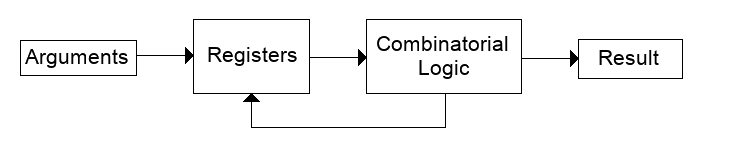
\includegraphics[keepaspectratio=true,scale=0.5]{img/recursion.png}
        \end{figure}
    }
\end{frame}


\begin{frame}[fragile]
    \frametitle{Higher-Order Functions --- Introduction}

    \begin{small}
    \begin{tabularx}{\textwidth}{c l l}
        \toprule
        Order        & Haskell                  & C
        \\ \midrule

        0            & \texttt{f :: Int}        & \texttt{int f()\{return 0;\}}
        \\ \midrule

        \only<2->{
            1            & \texttt{f :: Int -> Int} & \texttt{int f(int);}
            \\ \midrule
        }

        \only<3->{
            2            & \tiny{\texttt{f :: (Int -> Int) -> (Int -> Int)}} &
            \parbox{\textwidth}{%
                \tiny{\texttt{typedef int (*int2int)(int);}} \\
                \tiny{\texttt{int2int f(int2int);}}
            }
        \\ \bottomrule
        }
    \end{tabularx}
    \end{small}

    \pause[4]
    \lstinputlisting{src/flip.hs}
    \begin{lstlisting}
--Equivalent to:
revsub x y = y - x
    \end{lstlisting}
\end{frame}


\begin{frame}
    \frametitle{Higher-Order List Functions}
    \begin{itemize}
        \item List functions
            \begin{tabularx}{\textwidth}{l l l}
                \texttt{map}     & --- & Applies a function to each element of a list  \\
                \texttt{zipWith} & --- & Map generalized to two arguments/lists        \\
                \texttt{mfoldr}  & --- & Reduce a list of elements to a single value   \\
            \end{tabularx}

        \item Parallelism operator: \texttt{list ||| N}
    \end{itemize}
\end{frame}

\begin{frame}
    \frametitle{List Functions --- Maps}
    \lstinputlisting{src/map.hs}
    \lstinputlisting[language=C]{src/map.c}
    \begin{figure}
        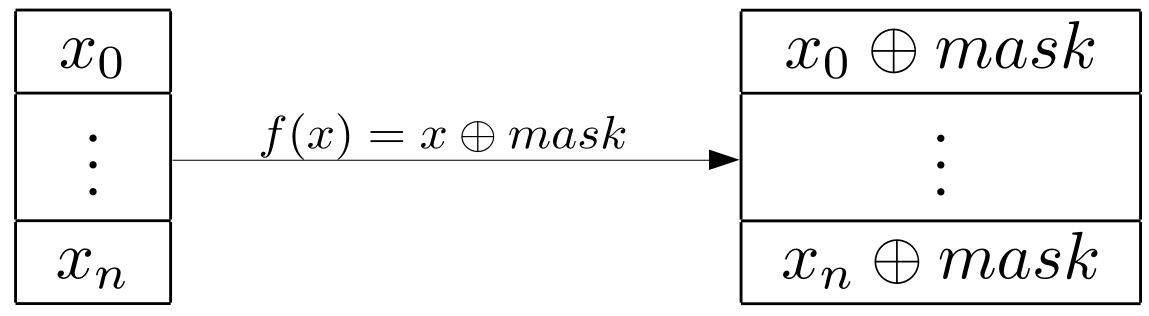
\includegraphics[keepaspectratio=true,scale=0.2]{src/map.png}
    \end{figure}
\end{frame}


\begin{frame}[t]
    \frametitle{List Functions --- Folds/Reduce}
    \begin{itemize}
        \item Problem:  Traditional folds are sequential
        \item Solution: Define a new kind of fold
    \end{itemize}

    \begin{small}
    \only<1-1>{
        \lstinputlisting[language=C]{src/fold.c}

        \begin{figure}
            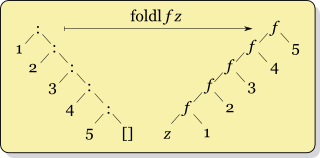
\includegraphics[keepaspectratio=true,scale=0.5]{img/fold.png}
            \caption{\tiny{Image: Cale Gibbard (21 October 2006). \textit{Left fold transformation} [Image]. Retrieved from
                    \newline \url{http://www.haskell.org/wikiupload/5/5a/Left-fold-transformation.png}.}}
        \end{figure}
    }
    \end{small}

    \only<2->{
        \begin{itemize}
            \item Monoidic Folds
                \begin{itemize}
                    \item Monoid --- a algebraic structure consisting of a function and a set over which it is associative and
                        has a right-identity.
                    \item This means that we can insert the right-identity at arbitrary points in the list, without changing the
                        result.
                    \item $\implies$ We can use reduction trees!
                    \item Added bonus: doesn't matter if the parallelism is a factor of the list length
                \end{itemize}
        \end{itemize}
    }
\end{frame}


\section{Case Study --- Dot Product}

\begin{frame}[fragile]
    \frametitle{Idiomatic C}

\begin{lstlisting}[language=C]
int dotProduct(const int* __restrict__ listA, const int* __restrict__ listB, int length){
    int result = 0;

    #pragma unroll_loop_with_parallelism 3
    for(int i = 0; i < length; i++)
        result += listA[i] * listB[i];

    return result;
}
\end{lstlisting}
\end{frame}

\begin{frame}[fragile]
    \frametitle{With Separate Addition and Multiplication}

\begin{lstlisting}[language=C]
int dotProduct(const int* __restrict__ listA, const int* __restrict__ listB, int length){
    int result = 0;
    int tmp[length];

    #pragma unroll_loop_with_parallelism 3
    for(int i = 0; i < length; i++)
        tmp[i] = listA[i] * listB[i];

    #pragma unroll_loop_with_parallelism 3
    for(int i = 0; i < length; i++)
        result += tmp[i];

    return result;
}
\end{lstlisting}
\end{frame}

\begin{frame}[fragile]
    \frametitle{Generalized to arbitrary functions}

\begin{lstlisting}[language=C]
int innerProd(const int* __restrict__ listA, const int* __restrict__ listB, int length){
    int result = 0;
    int tmp[length];

    #pragma unroll_loop_with_parallelism 3
    for(int i = 0; i < length; i++)
        tmp[i] = func1(listA[i], listB[i]);

    #pragma unroll_loop_with_parallelism 3
    for(int i = 0; i < length; i++)
        result = func2(result, tmp[i]);

    return result;
}
\end{lstlisting}
\end{frame}

\begin{frame}[fragile]
    \frametitle{In Haskell}

\begin{lstlisting}
sum :: [Int] -> Int
sum = mfoldr (+) 0 ||| 3

dotProduct :: [Int] -> [Int] -> Int
dotProduct listA listB = sum $ zipWith (*) listA listB ||| 3
\end{lstlisting}

\begin{figure}
    \includegraphics[keepaspectratio=true,scale=0.2]{"img/Dot Product Block Diagram".pdf}
\end{figure}
\end{frame}

\begin{frame}
    \frametitle{In Haskell}
    \begin{figure}
        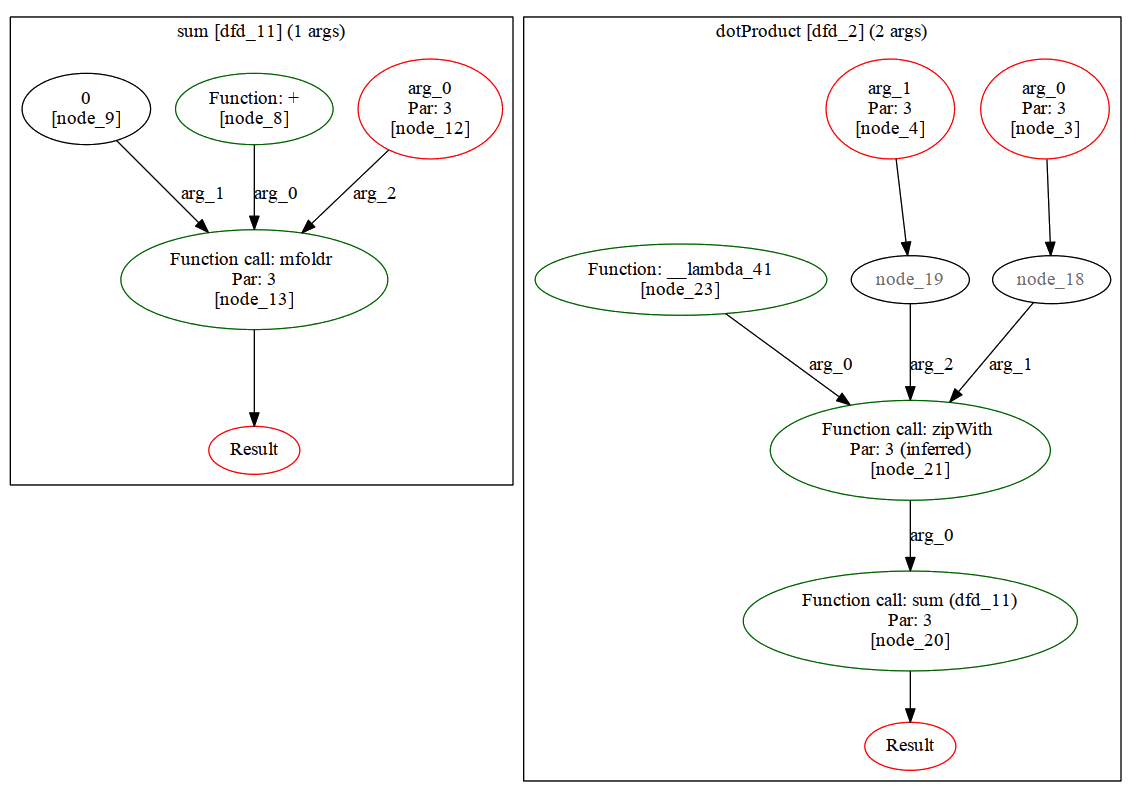
\includegraphics[keepaspectratio=true,scale=0.25]{img/dotProduct.png}
    \end{figure}
\end{frame}

\section{Future Work}

\begin{frame}
    \frametitle{Future Work}
    \begin{itemize}
        \item Improved type support
            \begin{itemize}
                    \item Variable width integers
                    \item Fixed-point types
                    \item Nested lists
            \end{itemize}

        \item Complete type \& parallelism inference
        \item Closures
        \item Compilation of recursive list functions
        \item Resource sharing
    \end{itemize}
\end{frame}


\begin{frame}
    \frametitle{Demo \& Questions}
\end{frame}

\end{document}

